\documentclass{article}\usepackage[]{graphicx}\usepackage[]{color}
%% maxwidth is the original width if it is less than linewidth
%% otherwise use linewidth (to make sure the graphics do not exceed the margin)
\makeatletter
\def\maxwidth{ %
  \ifdim\Gin@nat@width>\linewidth
    \linewidth
  \else
    \Gin@nat@width
  \fi
}
\makeatother

\definecolor{fgcolor}{rgb}{0.345, 0.345, 0.345}
\newcommand{\hlnum}[1]{\textcolor[rgb]{0.686,0.059,0.569}{#1}}%
\newcommand{\hlstr}[1]{\textcolor[rgb]{0.192,0.494,0.8}{#1}}%
\newcommand{\hlcom}[1]{\textcolor[rgb]{0.678,0.584,0.686}{\textit{#1}}}%
\newcommand{\hlopt}[1]{\textcolor[rgb]{0,0,0}{#1}}%
\newcommand{\hlstd}[1]{\textcolor[rgb]{0.345,0.345,0.345}{#1}}%
\newcommand{\hlkwa}[1]{\textcolor[rgb]{0.161,0.373,0.58}{\textbf{#1}}}%
\newcommand{\hlkwb}[1]{\textcolor[rgb]{0.69,0.353,0.396}{#1}}%
\newcommand{\hlkwc}[1]{\textcolor[rgb]{0.333,0.667,0.333}{#1}}%
\newcommand{\hlkwd}[1]{\textcolor[rgb]{0.737,0.353,0.396}{\textbf{#1}}}%
\let\hlipl\hlkwb

\usepackage{framed}
\makeatletter
\newenvironment{kframe}{%
 \def\at@end@of@kframe{}%
 \ifinner\ifhmode%
  \def\at@end@of@kframe{\end{minipage}}%
  \begin{minipage}{\columnwidth}%
 \fi\fi%
 \def\FrameCommand##1{\hskip\@totalleftmargin \hskip-\fboxsep
 \colorbox{shadecolor}{##1}\hskip-\fboxsep
     % There is no \\@totalrightmargin, so:
     \hskip-\linewidth \hskip-\@totalleftmargin \hskip\columnwidth}%
 \MakeFramed {\advance\hsize-\width
   \@totalleftmargin\z@ \linewidth\hsize
   \@setminipage}}%
 {\par\unskip\endMakeFramed%
 \at@end@of@kframe}
\makeatother

\definecolor{shadecolor}{rgb}{.97, .97, .97}
\definecolor{messagecolor}{rgb}{0, 0, 0}
\definecolor{warningcolor}{rgb}{1, 0, 1}
\definecolor{errorcolor}{rgb}{1, 0, 0}
\newenvironment{knitrout}{}{} % an empty environment to be redefined in TeX

\usepackage{alltt}
\usepackage[sc]{mathpazo}
\renewcommand{\sfdefault}{lmss}
\renewcommand{\ttdefault}{lmtt}
\usepackage[T1]{fontenc}
\usepackage{geometry}
\geometry{verbose,tmargin=2.5cm,bmargin=2.5cm,lmargin=2.5cm,rmargin=2.5cm}
\setcounter{secnumdepth}{2}
\setcounter{tocdepth}{2}
\usepackage[unicode=true,pdfusetitle,
 bookmarks=true,bookmarksnumbered=true,bookmarksopen=true,bookmarksopenlevel=2,
 breaklinks=false,pdfborder={0 0 1},backref=false,colorlinks=false]
 {hyperref}
\hypersetup{
 pdfstartview={XYZ null null 1}}

\makeatletter
%%%%%%%%%%%%%%%%%%%%%%%%%%%%%% User specified LaTeX commands.
\renewcommand{\textfraction}{0.05}
\renewcommand{\topfraction}{0.8}
\renewcommand{\bottomfraction}{0.8}
\renewcommand{\floatpagefraction}{0.75}

\makeatother
\IfFileExists{upquote.sty}{\usepackage{upquote}}{}
\begin{document}



\title{ My short analysis}

\author{ Vijay%
\thanks{This report is automatically generated with the R package \textbf{knitr}
        (version 1.15.1).}}

\maketitle
The results below are generated from an R script.

\begin{knitrout}
\definecolor{shadecolor}{rgb}{0.969, 0.969, 0.969}\color{fgcolor}\begin{kframe}
\begin{alltt}
\hlcom{# First we load the packages}
\hlkwd{library}\hlstd{(tidyr)}
\hlkwd{library}\hlstd{(ggplot2)}

\hlstd{pers_exp} \hlkwb{<-} \hlstd{USPersonalExpenditure}

\hlcom{# Let's look at the data}
\hlstd{pers_exp}        \hlcom{#it looks like the row names are not actually in the matrix}
\end{alltt}
\begin{verbatim}
##                       1940   1945  1950 1955  1960
## Food and Tobacco    22.200 44.500 59.60 73.2 86.80
## Household Operation 10.500 15.500 29.00 36.5 46.20
## Medical and Health   3.530  5.760  9.71 14.0 21.10
## Personal Care        1.040  1.980  2.45  3.4  5.40
## Private Education    0.341  0.974  1.80  2.6  3.64
\end{verbatim}
\begin{alltt}
                \hlcom{#let's fix that}

\hlstd{expenditure_type} \hlkwb{<-} \hlkwd{rownames}\hlstd{(pers_exp)}
\hlstd{expenditure_type} \hlkwb{<-} \hlkwd{gsub}\hlstd{(} \hlstr{' '} \hlstd{,} \hlstr{'_'} \hlstd{, expenditure_type)}
\hlkwd{rownames}\hlstd{(pers_exp)} \hlkwb{<-} \hlkwa{NULL}
\hlstd{pers_exp} \hlkwb{<-} \hlkwd{as.data.frame}\hlstd{(pers_exp)}
\hlstd{pers_exp} \hlkwb{<-} \hlkwd{cbind}\hlstd{(expenditure_type,pers_exp)}

\hlcom{# Let's look at the data now}
\hlstd{pers_exp}        \hlcom{#better, but it doesn't look tidy to me}
\end{alltt}
\begin{verbatim}
##      expenditure_type   1940   1945  1950 1955  1960
## 1    Food_and_Tobacco 22.200 44.500 59.60 73.2 86.80
## 2 Household_Operation 10.500 15.500 29.00 36.5 46.20
## 3  Medical_and_Health  3.530  5.760  9.71 14.0 21.10
## 4       Personal_Care  1.040  1.980  2.45  3.4  5.40
## 5   Private_Education  0.341  0.974  1.80  2.6  3.64
\end{verbatim}
\begin{alltt}
                \hlcom{#let's fix that}


\hlstd{pers_exp} \hlkwb{<-} \hlkwd{gather}\hlstd{( pers_exp , `1940` , `1945` , `1950` , `1955` , `1960` ,}
        \hlkwc{key} \hlstd{= year,} \hlkwc{value} \hlstd{=  expenditure)}
\hlstd{pers_exp} \hlkwb{<-} \hlkwd{spread}\hlstd{( pers_exp ,} \hlkwc{key} \hlstd{= expenditure_type ,} \hlkwc{value} \hlstd{= expenditure)}

\hlcom{# Let's look at the data now}
\hlstd{pers_exp}        \hlcom{#better}
\end{alltt}
\begin{verbatim}
##   year Food_and_Tobacco Household_Operation Medical_and_Health Personal_Care
## 1 1940             22.2                10.5               3.53          1.04
## 2 1945             44.5                15.5               5.76          1.98
## 3 1950             59.6                29.0               9.71          2.45
## 4 1955             73.2                36.5              14.00          3.40
## 5 1960             86.8                46.2              21.10          5.40
##   Private_Education
## 1             0.341
## 2             0.974
## 3             1.800
## 4             2.600
## 5             3.640
\end{verbatim}
\begin{alltt}
\hlcom{# Plot private education over time}
\hlkwd{ggplot}\hlstd{( pers_exp ,} \hlkwd{aes}\hlstd{( year , Private_Education))}\hlopt{+}
        \hlkwd{geom_bar}\hlstd{(}\hlkwc{stat}\hlstd{=}\hlstr{'identity'}\hlstd{)}\hlopt{+}
        \hlkwd{labs}\hlstd{(} \hlkwc{x} \hlstd{=} \hlstr{'Year'} \hlstd{,} \hlkwc{y} \hlstd{=} \hlstr{'Expenditure on private education\textbackslash{}nin billions of $'}\hlstd{)} \hlopt{+}
        \hlkwd{theme_classic}\hlstd{()}
\end{alltt}
\end{kframe}

{\centering 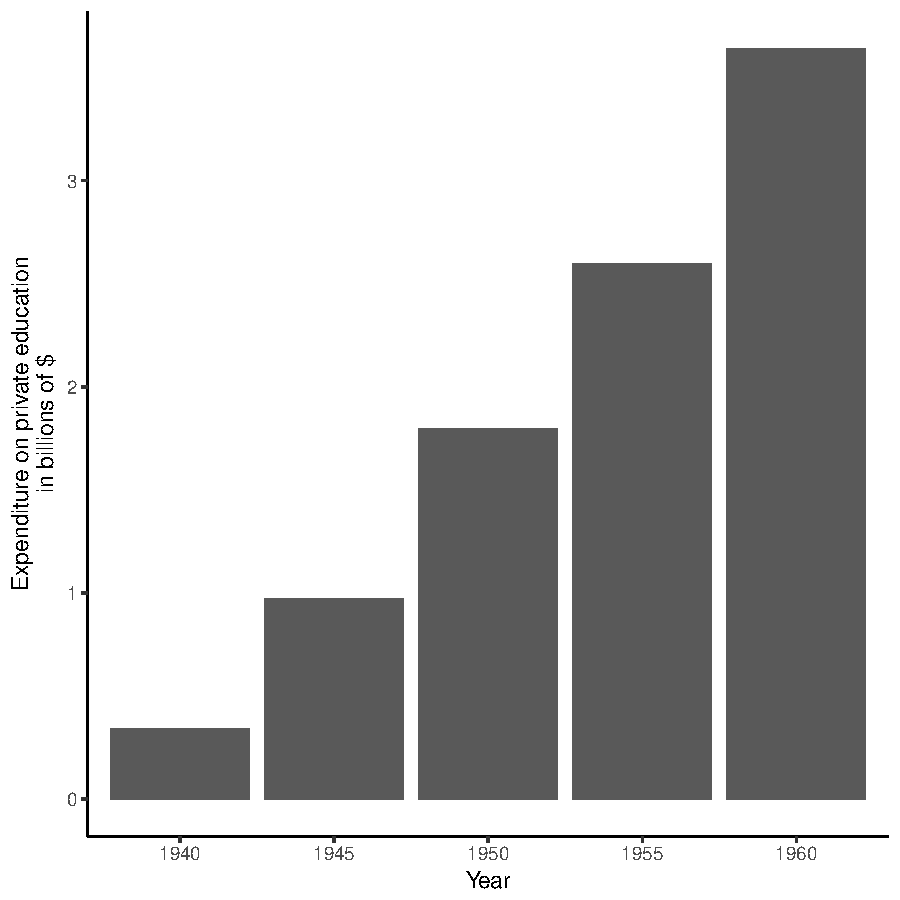
\includegraphics[width=.6\linewidth]{figure/my-simple-report-Rnwauto-report-1} 

}



\end{knitrout}

The R session information (including the OS info, R version and all
packages used):

\begin{knitrout}
\definecolor{shadecolor}{rgb}{0.969, 0.969, 0.969}\color{fgcolor}\begin{kframe}
\begin{alltt}
\hlkwd{sessionInfo}\hlstd{()}
\end{alltt}
\begin{verbatim}
## R version 3.3.2 (2016-10-31)
## Platform: x86_64-pc-linux-gnu (64-bit)
## Running under: Ubuntu 16.04.2 LTS
## 
## locale:
##  [1] LC_CTYPE=en_GB.UTF-8       LC_NUMERIC=C               LC_TIME=en_GB.UTF-8       
##  [4] LC_COLLATE=en_GB.UTF-8     LC_MONETARY=en_GB.UTF-8    LC_MESSAGES=en_GB.UTF-8   
##  [7] LC_PAPER=en_GB.UTF-8       LC_NAME=C                  LC_ADDRESS=C              
## [10] LC_TELEPHONE=C             LC_MEASUREMENT=en_GB.UTF-8 LC_IDENTIFICATION=C       
## 
## attached base packages:
## [1] stats     graphics  grDevices utils     datasets  methods   base     
## 
## other attached packages:
##  [1] Hmisc_4.0-1     Formula_1.2-1   survival_2.40-1 lattice_0.20-34 gdtools_0.1.4  
##  [6] psych_1.6.12    tidyr_0.6.1     knitr_1.15.1    plotly_4.5.6    ggplot2_2.2.1  
## 
## loaded via a namespace (and not attached):
##  [1] Rcpp_0.12.10        RColorBrewer_1.1-2  plyr_1.8.4          highr_0.6          
##  [5] base64enc_0.1-3     tools_3.3.2         rpart_4.1-10        base64_2.0         
##  [9] digest_0.6.12       htmlTable_1.7       jsonlite_1.1        evaluate_0.10      
## [13] tibble_1.2          gtable_0.2.0        viridisLite_0.1.3   Matrix_1.2-7.1     
## [17] DBI_0.6             yaml_2.1.14         parallel_3.3.2      gridExtra_2.2.1    
## [21] cluster_2.0.5       dplyr_0.5.0         httr_1.2.1          stringr_1.2.0      
## [25] htmlwidgets_0.8     nnet_7.3-12         grid_3.3.2          data.table_1.10.0  
## [29] svglite_1.2.0       R6_2.2.0            tcltk_3.3.2         foreign_0.8-67     
## [33] latticeExtra_0.6-28 reshape2_1.4.2      purrr_0.2.2         magrittr_1.5       
## [37] scales_0.4.1        htmltools_0.3.5     splines_3.3.2       assertthat_0.1     
## [41] mnormt_1.5-5        colorspace_1.3-2    labeling_0.3        stringi_1.1.2      
## [45] acepack_1.4.1       openssl_0.9.5       lazyeval_0.2.0      munsell_0.4.3
\end{verbatim}
\begin{alltt}
\hlkwd{Sys.time}\hlstd{()}
\end{alltt}
\begin{verbatim}
## [1] "2017-03-24 00:03:03 GMT"
\end{verbatim}
\end{kframe}
\end{knitrout}


\end{document}
